Механизм Викри-Кларка-Гровса основан на \textit{интервенции}. Для выяснения стоимости представляется мнимая (counterfactual) ситуация, в которой победитель не участвовал в аукционе.

\begin{figure}[h]
    \centering
    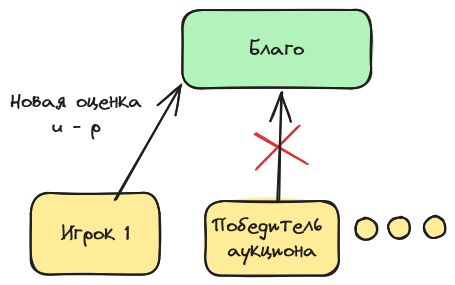
\includegraphics[width=0.5\textwidth]{assets/mechanism/vcg.excalidraw.png}
    \caption{Механизм Викри-Кларка-Гровса задает доверительный механизм распределения ресурсов.}
    \label{mech}
\end{figure}


 Идея VCG-аукциона состоит в том, что каждый участник аукциона платит цену исходя из того, как его участие воздействует на всех остальных участников. 